\documentclass[light]{lutbeamer} % change between light and dark for the background
%\documentclass[t]{lutbeamer} % use "t" option for top alignment 
\usepackage{caption}
\usepackage{xcolor}
\captionsetup{labelfont={color=gr},textfont={color=gr}}
\DeclareCaptionLabelFormat{nocolon}{#1 #2}
\captionsetup{labelformat=nocolon}
\usepackage{pgfpages}
\usepackage{amssymb}
\usepackage{amsmath}
\usepackage{tabularx}
\usepackage{array}
\usepackage{adjustbox}
\usepackage{hyperref} % Link
\usepackage{bm}
\usepackage{amsfonts}
\usepackage{algorithmic}
\usepackage{textcomp}
\usepackage{xcolor}
\usepackage{algorithm} 
\usepackage{amsthm} % add this package to use the definition environment

\setbeameroption{hide notes} % Only slides
% \setbeameroption{show only notes} % Only notes
% \setbeameroption{show notes on second screen=right} % Both


% Define the custom color using hexadecimal code
\definecolor{customcolor}{HTML}{123363}

% Define a new block environment with a custom background color and white text
\newenvironment{customblock}{%
    \setbeamercolor{block body}{bg=customcolor,fg=white}%
    \begin{block}%
}{%
    \end{block}%
}


\setdepartment{Data Science and Analytics Thrust, Information Hub}
\institute[HKUSTGZ]{The Hong Kong University of Science and Technology (Guangzhou)}
\author{Mingze Gong}
\title{Main Title}
\subtitle{This is a subtitle}
\date{\today}


\begin{document}

% % front page
% { % all template changes are local to this group.
% \setbeamertemplate{navigation symbols}{}
% \begin{frame}<article:0>[plain,noframenumbering]
%     \begin{tikzpicture}[remember picture,overlay]
%         \node[at=(current page.center)] {
%             \includegraphics[
%                 width=\paperwidth,
%                 height=\paperheight]{figures/GZ Campus.jpeg}
%         };
%     \end{tikzpicture}
% \end{frame}
% }

% Outline with figure on the right
\AtBeginSubsection[]
{
    \begin{frame}[plain,noframenumbering]
        \frametitle{Outline}
        \begin{columns}
            % Left column for the outline
            \begin{column}{0.6\textwidth}
                \tableofcontents[currentsection,
                    currentsubsection,
                    %hideothersubsections, 
                    %sectionstyle=show/shaded, 
                    %subsectionstyle=show/shaded%/hide
                ]
            \end{column}
            \hspace{-4em}
            % Right column for the figure
            \begin{column}{0.42\textwidth}
                \begin{figure}
                    \centering
                    \vspace{-2em}
                    \includegraphics[width=\textwidth]{logos/GZ Campus.pdf} % Adjust path and filename
                \end{figure}
            \end{column}
        \end{columns}
    \end{frame}
}


{ % title page
    \begin{frame}[plain]
        \maketitle
        \small
        \par\vskip-0.1em
        {\footnotesize
        \begin{beamercolorbox}[sep=8pt,left]{author}
            \usebeamerfont{author}{Presented by \insertauthor} on \insertdate
        \end{beamercolorbox}%\vskip0.5em
        }
    \end{frame}
}
% % % % % % % % % % % % % % % % % % % % % % % % % % % % % % % % % % % %
\section{Introduction}

\subsection{Research Overview}


\begin{frame}
    \frametitle{Introduction}
    \framesubtitle{DSTGCRN: Motivations and Contributions}
    \begin{columns}[T] % Aligns the top of the content in both columns
        \begin{column}{0.45\textwidth}
            \textbf{Motivations:}
            \begin{itemize}
                \item Overcome limitations of traditional methods in handling complex, dynamic environmental data.
                \item Leverage insights from the success of Graph Neural Networks (GNNs) in sectors such as traffic and energy to enhance spatial-temporal analysis.
            \end{itemize}
        \end{column}
        \begin{column}{0.45\textwidth}
            \textbf{Contributions:}
            \begin{itemize}
                \item Combines Graph Convolutional Networks (GCN) and Recurrent Neural Networks (RNN) to model evolving inter-regional relationships and spatial-temporal dynamics.
                \item Boosts predictive accuracy and offers comprehensive insights to guide environmental policy.
                \item Facilitates informed, real-time policy decisions adapted to specific regional contexts.
            \end{itemize}
        \end{column}
    \end{columns}
\end{frame}

\subsection{Literature Review}

\begin{frame}
    \frametitle{Literature Review}
    \framesubtitle{Statistical and Machine Learning Approaches}
    \begin{itemize}
        \item \textbf{Statistical Methods:}
              \begin{itemize}
                  \item \textbf{ARIMA Models:} Employed for time series forecasting; adjusts for trends and seasonality.
                  \item \textbf{Grey Forecasting Models (GM):} Effective under conditions of limited or incomplete data, applicable in emerging markets.
                  \item \textbf{Hybrid Models:} Combining GM and ARIMA to address non-linear and non-stationary data, enhancing forecast accuracy.
              \end{itemize}
        \item \textbf{Machine Learning Methods:}
              \begin{itemize}
                  \item \textbf{Deep Learning:} Excels in learning complex data patterns, significantly improving prediction capabilities.
                  \item \textbf{Hybrid Approaches:} Integration of neural networks with statistical methods boosts accuracy and reliability.
                  \item \textbf{Regional Variability:} Challenges include accommodating diverse environmental conditions, impacting scalability and model performance.
              \end{itemize}
    \end{itemize}
\end{frame}


% % % % % % % % % % % % % % % % % % % % % % % % % % % % % % % % % % % %
% % % % % % % % % % % % % % % % % % % % % % % % % % % % % % % % % % % %
% % % % % % % % % % % % % % % % % % % % % % % % % % % % % % % % % % % %
% % % % % % % % % % % % % % % % % % % % % % % % % % % % % % % % % % % %
% % % % % % % % % % % % % % % % % % % % % % % % % % % % % % % % % % % %
% % % % % % % % % % % % % % % % % % % % % % % % % % % % % % % % % % % %
% % % % % % % % % % % % % % % % % % % % % % % % % % % % % % % % % % % %
% % % % % % % % % % % % % % % % % % % % % % % % % % % % % % % % % % % %

\appendix % to start a separate page numbering

\section*{Bibliography}
\begin{frame}[allowframebreaks]
    \textbf{References}
    \printbibliography
\end{frame}


{ % all template changes are local to this group.
\setbeamertemplate{navigation symbols}{}
\begin{frame}<article:0>[plain,noframenumbering]
    \begin{tikzpicture}[remember picture,overlay]
        \node[at=(current page.center)] {
            
\includegraphics[
                width=\paperwidth,
                height=\paperheight]{logos/ThankYouPage.png}
        };
    \end{tikzpicture}
    % \begin{tikzpicture}[remember picture,overlay]
    %     \node[at=(current page.center)] {
    %         
\includegraphics[keepaspectratio,
    %             width=0.65\paperwidth,
    %             height=\paperheight]{figures/ThankYouPage.png}
    %     };
    % \end{tikzpicture}
\end{frame}
}

\end{document}
